%%%%%%%%%%%%%%%%%%%%%%%%%%%%%%%%%%%%%%%%%%%%%%%%%%%%%%%%%%%%%%%%%%%%%%%%%%%%%%%
%% University of Ulm
%%
%% Faculty of Engineering and Computer Science
%% Institute of Measurement, Control and Microtechnology
%%
%%
%% Template for Student Research Projects, Diploma, Bachelor and Master Thesis
%%
%% by order of Dr.-Ing. Michael Buchholz
%% created by Stephan Grensemann 2010
%%%%%%%%%%%%%%%%%%%%%%%%%%%%%%%%%%%%%%%%%%%%%%%%%%%%%%%%%%%%%%%%%%%%%%%%%%%%%%%

\documentclass[]{mrmthesis}     % <-- [your options (see docu)]
%defaults if no options are used: language=de, Master Thesis, confidential=false,namebehindauthortitle=false,

%new since version 1.6: option "namebehindauthortitle" for author title in front of name,
%   new default is title behind name
%Example:  \documentclass[namebehindauthortitle]{mrmthesis} % for title like "Dipl.-Ing. (FH)"

%new since version v1.6: use of biber instead of bibtex8 to generate biblatex labels (i.e. biblatex backend)
%   please set new option "backendbibtex=true" if bibtex8 is used (not recommended, not longer supported)
%   if biber is not part of your (La)TeX distribution, you can get it from http://biblatex-biber.sourceforge.net/

%new since version 1.4: option "confidential" for theses which should not be published
%Example:  \documentclass[confidential]{mrmthesis}

%2015/05/11 v. 1.9b Uni Ulm - Measurement, Control and Microtechnology
%%%%%%%%%%%%%%%%%%%%%%%%%%%%%%%%%%%%%%%%%%%%%%%%%%%%%%%%%%%%%%%%%%%%%%%%%%%%%%%
%loading extra packages / short list of recommended packages

\usepackage{fixltx2e}                  %fix problems in LaTeX that it "`would be nice"' to correct before next LaTeX release

%note: AMSmath Package is already loaded by mrmthesis to avoid problems with hyperref

%\usepackage{amssymb}                   %special characters in AMS
%\usepackage{amsfonts}                  %TeX fonts from the American Mathematical Society
%\usepackage{dsfont}                    %Doublestroke Font for set symbols, e.g. real numbers \mathds{R}
%\usepackage{amsbsy}                    %producing bold mathematics symbols where appropriate fonts exist
%\usepackage{mathrsfs}                  %Support use of the Raph Smith�s Formal Script font in mathematics
%\usepackage{mathdots}                  %Commands to produce dots in math that respect font size
%\usepackage{upgreek}                   %provides upright greek letters

%\usepackage{siunitx}                   %International System of Units
%\usepackage{textcomp}                  %provide many text symbols in the TS1 encoding

%\usepackage{xspace}                    %provides a single command that looks at what comes after it in the command stream,
                                        %and decides whether to insert a space to replace one "eaten" by the TeX command decoder

%\usepackage{float}                     %improved interface for floating objects
%\usepackage{rotating}                  %rotation tools, including rotated full-page floats

%\usepackage{ltxtable}                  %merged tabularx - longtable package
%\usepackage{booktabs}                  %publication quality tables in LaTeX

%\usepackage{listings}                  %Typeset source code listings using LaTeX
%\lstset{language=html,%
%           frameround=fttt,%
%           breaklines=true,%
%           numbers=left,%
%           numberbychapter=true,%
%           captionpos=b,%
%           basicstyle=\scriptsize}%

%%OLD:
%\usepackage{pstricks}                  %set of macros that allow the inclusion of PostScript drawings directly inside LaTeX code
%\usepackage{auto-pst-pdf}              %Package for using pstricks/PSfrag with PDF(La)TeX, requires PERL!
                           % PLEASE NOTE: to use this package you have to add
                           %  "`--enable-write18"' as compiler argument in the
                           %  LaTeX => PDF output-profile (see description in docu)
%
%IF MODIFICATION OF EPS FILES IS NECESSARY, BETTER USE THE NEW PACKAGE pstool
%\usepackage{pstools}
                           % PLEASE NOTE: to use this package you have to add
                           %  "`--enable-write18"' as compiler argument in the
                           %  LaTeX => PDF output-profile (see description in docu)
%
%THE BEST SOLUTION: USE pgfplots/tikz INSTEAD OF EPS FILES (see also tool "matlab2tikz")
%\usepackage{tikz}                      %language for producing vector graphics from a geometric/algebraic description
%\usepackage{pgfplots}                  %draws high-quality function plots in normal or logarithmic scaling

%\usepackage{epstopdf}                  %convert EPS to 'encapsulated' PDF using GhostScript
                           % PLEASE NOTE: to use this package you have to add
                           %  "`--enable-write18"' as compiler argument in the
                           %  LaTeX => PDF output-profile (see description in docu)

%\usepackage{nomencl}                   %produce lists of symbols as in nomenclature
%\ifthenelse{\boolean{en}}{}{\renewcommand{\nomname}{Nomenklatur}}
%\makenomenclature

%%%%%%%%%%%%%%%%%%%%%%%%%%%%%%%%%%%%%%%%%%%%%%%%%%%%%%%%%%%%%%%%%%%%%%%%%%%%%%%

%!!!
%Regarding the compatibility for different platforms and LATEX distributions, the mrmthesis class requires
% "latin1" (ISO 8859-1) encoding of all files. Especially UNIX user should ensure this encoding using the
% options of your preferred editor.
%!!!

%--------------------------------------------------------------
%% set options for mrmbibstyle:
%% url, ISBN, eprint, DOI: content of respective field is never printed if set to false (default)
%% printlanguage: if set to false (default), the language field is never printed. set to true and use standard
%%      biblatex option clearlang to print language fielf for specific languages (see biblatex manual)
%% yearonly: if set true (default), do not print day or month of a publication even if given
%% titlesentencecase: If set to false (default), all titles are written as given in the bib file. If set to true,
%%      all titles of articels, inproceedings etc. (but not booktitle etc.) are transformed to sentence case,
%%      i.e. only the first letter of the title is capital, all other words start with small letters even if
%%      capital letters in the bib file. Use additional curly braces e.g. for abbreviations which should
%%      remain capital letters (as in original bibtex). The command has no effect on entries where the entry
%%      field "hyphenation" is set to e.g. "ngerman".
\ExecuteBibliographyOptions{eprint=false, url=false, isbn=false, doi=false, yearonly=true, printlanguage=false, titlesentencecase=false}

%\ExecuteBibliographyOptions{firstinits=true} %activate, if all given names shall be abbreviated to initials

%%Use field hyphenation for bib entries to set the language of the bib entry, e.g. for correct hyphenation.
%%Do not mix up with the hyphenation command below!
\ExecuteBibliographyOptions{babel=hyphen} %uses hyphenation for language given in entry's hyphenation field (or global language otherwise)


%% Using new command to add bib file, set options for not printing
\addbibresource{my_mrmthesis.bib} % <- type in your bibfile

%% If the above does not work with older versions of biblatex,
%% try the compatibility mode using the folling command instead:
%\bibliography{my_mrmthesis}      % <- type in your bibfile
%--------------------------------------------------------------

%\hyphenation{}                         %insert hyphenations for unknown words


%Datei f�r eigene Kommandos, z.B.


%Typographie: (ben�tigen Package xspace)
%\newcommand{\dasheisst}{\mbox{d.\,h.}\xspace}
%\newcommand{\unteranderem}{\mbox{u.\,a.}\xspace}
%\newcommand{\zumbeispiel}{\mbox{z.\,B.}\xspace}

%Befehl f�r deutsche Anf�hrungszeichen: (ben�tigt babel mit (n)german)
%\shorthandon{"} %bei Einbindung der Command-Datei vor \begin{document} n�tig
%\newcommand{\gq}[1]{"`#1"'} %doppelte Anf�hrungszeichen, Verwendung \gq{in Anf�hrungszeichen}
%\newcommand{\sgq}[1]{\glq #1\grq{}} %einfache Anf�hrungszeichen, Verwendung \sgq{in Anf�hrungszeichen}
%\shorthandoff{"} %bei Einbindung der Command-Datei vor \begin{document} n�tig


%Mathematisches
%%%%%%%%%%%%%%%
%
%Befehl \vm zur Notation von Vektoren und Matrizen in Fettschrift
%\newcommand{\vm}[1]{\protect\ensuremath\boldsymbol{#1}} %ben�tigt Paket amsbsy
%Befehl \vm zur Notation von Vektoren und Matrizen mit Unterstrich:
%\newcommand{\vm}[1]{\protect\ensuremath\underline{#1}}

%Befehl \trans f�r korrekt gesetztes "T" im Mathemodus f�r "Transponiert
%\newcommand{\trans}{^\text{\rm \textup{T}}} %Verwendung: \vm A\trans
%�hnliche Befehle:
%\newcommand{\inv}{^{-1}} %Inverse
%\newcommand{\pinv}{^{\dag}} %Pseudoinverse
%\newcommand{\opt}{\ensuremath ^\star} %Optimale L�sung

%angepasste Versionen f�r optisch besseren Satz bei einigen Buchstaben (z.B. Y,A):
%\newcommand{\transnah}{^{\!\text{\rm \textup{T}}}}
%\newcommand{\invnah}{^{\!-1}}
%\newcommand{\pinvnah}{^{\!\dag}}
%\newcommand{\optnah}{\ensuremath ^{\!\star}}


%aufrechtes "e" f�r die e-Funktion, als Argument die Potenz:
%\newcommand{\efkt}[1]{\ensuremath {{\rm e}}^{#1}}

%Formeln im Text ohne Zeilenumbruch:
%\newcommand{\teq}[1]{\mbox{$#1$}}

%Befehl f�r PT_n-Glied:
%\newcommand{\PT}[1]{\teq{\text{PT}_{#1}}}

%Einheitsmatrix:
%\newcommand{\eye}[1]{\vm{I}}
%mit Dimension:
%%\newcommand{\eye}[1]{\vm{I}_{\!#1}}

%weitere mathematische Funktionen:
%\DeclareMathOperator{\trace}{spur}
%\DeclareMathOperator{\sign}{sign}
%\DeclareMathOperator{\diag}{diag}


%Normen:
%\newcommand{\frobnorm}[1]{\ensuremath \left\| #1 \right\|_\text{F}}
%\newcommand{\zweinorm}[1]{\ensuremath \left\| #1 \right\|_2}
%\newcommand{\vmnorm}[1]{\ensuremath \left\| #1 \right\|}
                   %insert file with self-defined commands. The file exists and contains many examples.

%%%%%%%%%%%%%%%%%%%%%%%%%%%%%%%%%%%%%%%%%%%%%%%%%%%%%%%%%%%%%%%%%%%%%%%%%%%%%%%
%please fill out the following required information
\title{Erkennung von dynamischen Objekten in Stereobilddaten}
%\descriptiontitle{title for thesis description page with different line-breaks, if necessary} % Default: \title
%\affirmationtitle{title for affirmation page with different line-breaks, if necessary} % Default: \title
\author[m]{Daniel Jung} %use optional argument [f] for female label, default is [m] for male
%\authortitle{B.\,Sc.} %default: None, please note: use class option namebehindauthortitle if title should be printed in front of the name
\supervisor[m]{M. Sc. Martin Herrmann} %use optional argument [f] for female label, default is [m] for male
\examiner{Prof. Dr.-Ing. Klaus Dietmayer}
\coexaminer{Prof. Dr. Frank Steiper}
\issuedate{01.05.2018}
\submissiondate{31.10.2018}
%\place{}                       %default: Ulm

%%%%since v. 1.4: Possible re-definition of phrases for "confidential"-option
%%%%please note: Normally, there should be no reason to change these phrases
%%%% and changing can cause unwanted behaviour.
%%%\confidentialMainText{}
%%%\confidentialSubText{}

%%%%%%%%%%%%%%%%%%%%%%%%%%%%%%%%%%%%%%%%%%%%%%%%%%%%%%%%%%%%%%%%%%%%%%%%%%%%%%%
%main text
\begin{document}
% - - - - - - - - - - - - - - -
 \frontmatter
\maketitle
%  \projectdescription{\input{doc/projectdescription}}   % the file "projectdescription.tex" should be provided by your supervisor
  \affirmation

  %\extrafrontchapter{Foreword}{type in your text here} %or some other optional stuff
  %\extrafrontchapter{Thanks}{type in your text here}

  \tableofcontents
  %\listoffigures
  %\listoftables
  %\printnomenclature        %PLEASE NOTE: If you don't change the MakeIndex argument
                             % in the output-profile into
                             % "%bm.nlo" -s nomencl.ist -o "%bm.nls", no output will be produced
% - - - - - - - - - - - - - - -
 \mainmatter                       %import chapters (tip: use one tex-file for each chapter)
    \chapter{Bildverarbeitung}
\section{Boxfilter}
Boxfilter
Faltung
$$ \widetilde{I}(i, j)=I \ast f =  \sum_{\alpha=-m}^m \sum_{\beta=-n}^n I(i-\alpha, j-\beta) \cdot f(\alpha, \beta)$$
Relevant: 
$$ \sum_{\alpha=-m}^m \sum_{\beta=-n}^n f(\alpha, \beta) \stackrel{!}{=} 1 $$
Boxfilter - Mittelwertfilter
$$ f=\frac{1}{9} \begin{bmatrix} 1&1&1 \\ 1&1&1 \\ 1&1&1 \end{bmatrix}$$
$$ \widetilde{I}(i, j)=\frac{1}{9} \sum_{\alpha=-1}^1 \sum_{\beta=-1}^1 I(i-\alpha, j-\beta) $$
Veranschaulicht wird dieses Vorgehen in \ref{fig:boxfilter}. Im linken Abschnitt ist das Originalbild mit einem gr\"o\ss{}eren Objekt und einigen St\"orpixeln zu sehen. Im rechten Abschnitt ist die gefilterte Version zu sehen: Die einzelnen St\"orpixel im oberen Abschnitt des Bildes sind deutlich abgeschw\"acht. Die Grenzen des Objektes in der rechten, unteren Ecke sind jedoch ebenso verschwommen. Bei mehrfacher Anwendung eines Mittelwertfilters konvergieren alle Pixelwerte gegen den Mittelwert der Pixel des gesamten Bildes. Der Mittelwertfilter ist somit ein Tiefpassfilter und sorgt anschaulich daf\"ur, dass Bilder verschwimmen.
\begin{figure}
 \centering
 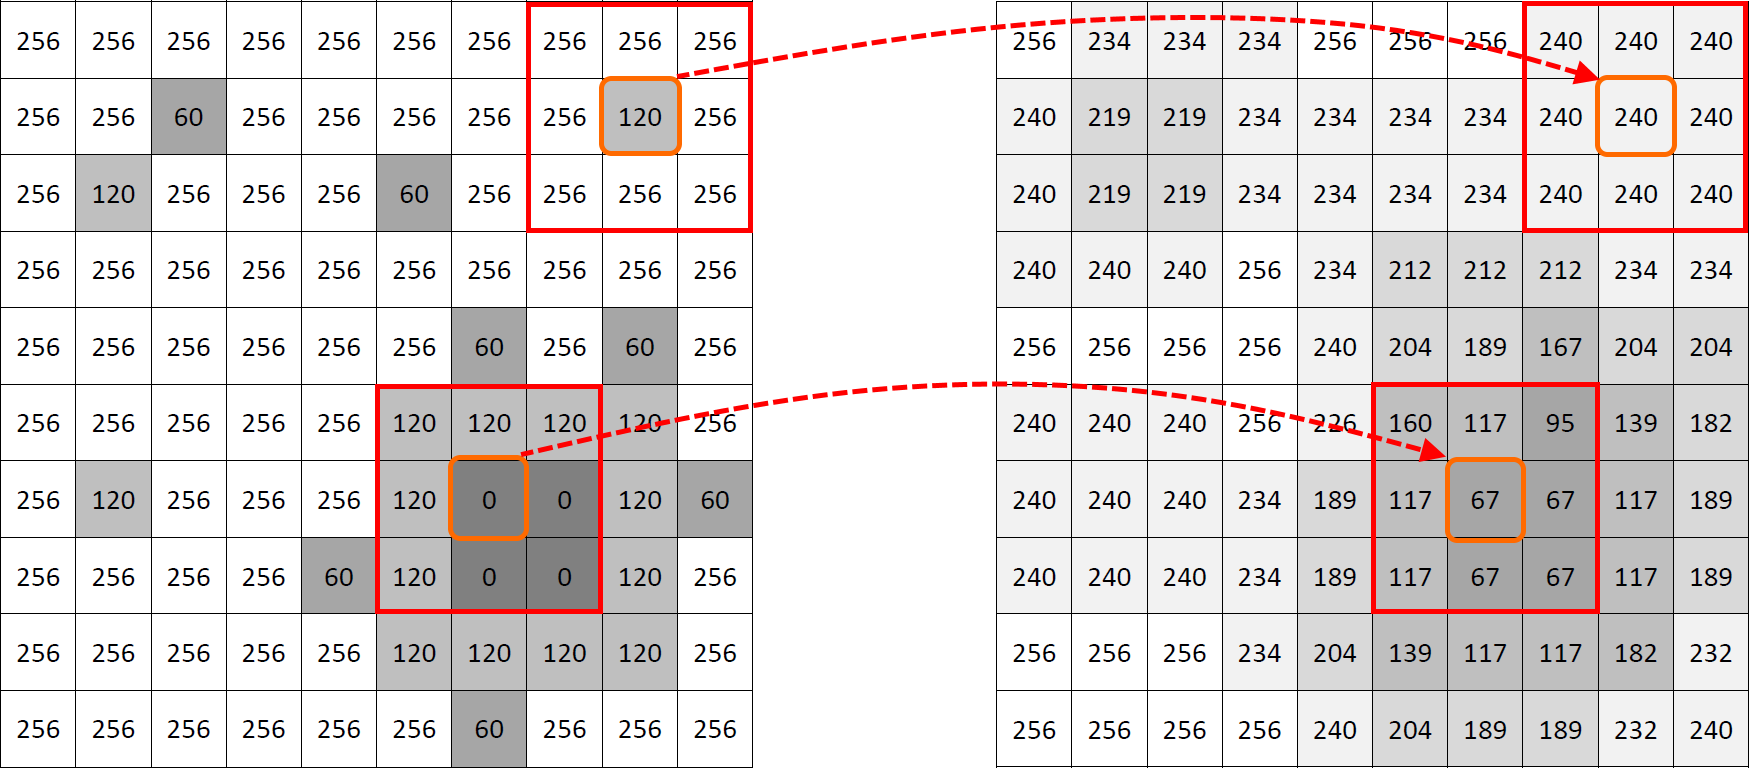
\includegraphics[width=1\textwidth]{media/filter/boxfilter_combined.png}
 \caption{Beispiel für 3x3 Boxfilter}
 \label{fig:boxfilter}
\end{figure}

Gau\ss{}filter:
\begin{equation}
 N(x, y) = \frac{1}{2\pi\sigma^2} e^{-\frac{x^2+y^2}{2\sigma^2}}
\end{equation}
Die Variable \( \sigma \) ergibt sich aus der Standardnormalverteilung mit \( \mu=0 \). Damit ergeben sich Filterkerne wie
\begin{multicols}{2}

\begin{equation*}
 G_{3x3}=\frac{1}{16} \begin{bmatrix} 1&2&1 \\ 2&4&2 \\ 1&2&1 \end{bmatrix}
\end{equation*}
 
 \columnbreak
 \begin{equation*}
 G_{5x5}=\frac{1}{256} \begin{bmatrix} 1&4&6&4&1 \\ 4&16&24&16&4 \\ 6&24&36&24&6 \\ 4&16&24&16&4 \\ 1&4&6&4&1 \end{bmatrix}
\end{equation*}
 
\end{multicols}

\section{Kantendetektion}

Sobelfilter zur Kantendetektion:
Analogie zentrale Differenz:
\begin{equation*}
 f^\prime (x)=\frac{f(x+\delta x)-f(x-\delta x)}{2\delta x}
\end{equation*}

\begin{multicols}{2}
\begin{align*}
 S_x &= \frac{1}{8} \begin{bmatrix}[r] -1&0&1 \\ -2&0&2 \\ -1&0&1 \end{bmatrix} \\
 S_u &= \frac{1}{8} \begin{bmatrix}[r] 0&-1&-2 \\ 1&0&-1 \\ 2&1&0 \end{bmatrix}
\end{align*}

\columnbreak

\begin{align*}
 S_y &= \frac{1}{8} \begin{bmatrix}[r] -1&-2&-1 \\ 0&0&0 \\ 1&2&1 \end{bmatrix} \\
 S_v &= \frac{1}{8} \begin{bmatrix}[r] -2&-1&0 \\ -1&0&1 \\ 0&1&2 \end{bmatrix}
\end{align*}
\end{multicols}

Canny Algorithmus: Berechne Kantenbild \(D(x, y)\) und Gradientenrichtung \( \phi(x, y) \)
\begin{eqnarray*}
D(x, y)=\sqrt{g_x(x, y)^2+g_y(x, y)^2} \\
\phi (x, y)= \tan^{-1}\bigg( \frac{g_y(x, y)}{g_x(x, y)} \bigg)
\end{eqnarray*}
Wegen 8er Nachbarschaft: Runden auf \( 45^\circ \)
\cite{imageprocessing_edgedetection}

\section{Interpolation}

Die Interpolation beschreibt die Suche nach einer Funktion, welche vorgebene Funktionswerte \( f_i \) an St\"utzstellen \( (x_i) \) am Besten approximiert. Im Falle der Bildbearbeitung l\"asst sich die Funktion beschreiben als 
\( f: \mathbb{R}^2\mapsto\mathbb{R}, f(x_n)=f_n, n=1...4 \). F\"ur die Bildverarbeitung bilden die St\"utzstellen \(x_i\) im Allgemeinen ein Rechteck in dessen Inneren interpoliert wird, was auch bei der Vorstellung der nachfolgenden Verfahren der Fall ist. 

\subsection*{Nearest-Neighbor-Interpolation}
Wie der Name suggeriert wird bei diesem Verfahren der Wert als Ergebnis der Interpolation zur\"uckgegeben, dessen St\"utzstelle den kleinsten Abstand zum angefragten Punkt hat. Als Norm f\"ur den Abstand wird hierbei h\"aufig die Euklidische Norm herangezogen, generell sind jedoch auch andere Arten nutzbar. 
\begin{equation*}
f: \mathbb{R}^2\mapsto\mathbb{R},f(x)=x_k,k=\underset{{l \in {1,..., 4}}}{arg\,min} (||x-x_l||)
\end{equation*}


\subsection*{Bilineare Interpolation}
Die bilineare Interpolation nutzt eine lineare Ansatzfunktion um Werte zwischen den St\"utzstellen zu berechnen. Im Gegensatz zur Nearest-Neighbor-Interpolation ist es hier vor der Auswertung der Funktion notwendig einige Parameter zu berechnen. 
\begin{eqnarray*}
 f: \mathbb{R}^2\mapsto\mathbb{R}, f(x, y)&=&\sum_{i=0}^1 \sum_{j=0}^1 a_{ij}x^iy^j \\
&=&a_{00}+a_{10}x+a_{01}y+a_{11}xy
\end{eqnarray*}

Durch L\"osen eines linearen Gleichungssystems k\"onnen die Parameter \(a_{ij} \) f\"ur die bilineare Interpolation berechnet werden. Das Gleichungssystem ergibt sich aus \( f(x_i, y_i)=f_i, i=1...4 \), welches die Funktionsparameter und Funktionswerte an den St\"utzstellen sind.
\begin{equation*}
 \begin{pmatrix}
  1 & x_0 & y_0 & x_0y_0 \\
  1 & x_1 & y_1 & x_1y_1 \\
  1 & x_2 & y_2 & x_2y_2 \\
  1 & x_3 & y_3 & x_3y_3
 \end{pmatrix}
 \begin{pmatrix}
  a_{00} \\ a_{10} \\ a_{01} \\ a_{11}
 \end{pmatrix}
 =
 \begin{pmatrix}
  f_0 \\ f_1 \\ f_2 \\ f_3
 \end{pmatrix}
\end{equation*}

\subsection*{Bikubische Interpolation}
Die bikubische Interpolation nutzt statt einer linearen eine kubische Ansatzfunktion. Die Funktion hat dann die folgende Form:
\begin{equation*}
 f: \mathbb{R}^2\mapsto\mathbb{R}, f(x, y)=\sum_{i=0}^3 \sum_{j=0}^3 a_{ij}x^iy^j
\end{equation*}
Die Parameter \(a_{ij} \) werden wie bei der linearen Interpolation durch ein lineares Gleichungssystem berechnet. Zus\"atzlich zu den Funktionswerten \(f_i\) an den St\"utzstellen \( (x_i, y_i) \) m\"ussen hier auch die Werte der Ableitungen \( f_x, f_y, f_{xy} \) bekannt sein um das Gleichungssystem l\"osen zu k\"onnen. Dieses hat resultierend aus der kubischen Ansatzfunktion eine Gr\"o\ss{}e von \( 16\times 16 \). 

In beiden F\"allen werden die Parameter \(a_{ij} \) analytisch berechnet um nicht zur Laufzeit eine Reihe von Gleichunssystemen L\"osen zu m\"ussen. Eine sinnvolle Vorverarbeitung projeziert zudem die St\"utzstellen \( (x_i, y_i), i=1..4 \) auf die Eckpunkte des Einheitsquadrats. Dies hat zur Folge, dass sich die Funktion \( f: \mathbb{R}^2\mapsto\mathbb{R} \) auf \( f: [0, 1]^2\mapsto\mathbb{R} \) reduziert und die Rechenzeit deutlich reduziert werden kann, da sich das Gleichungssystem zur Berechnung vereinfachen l\"asst.

\section{Morphologische Operationen}
Morphologische Operationen werden auf Bin\"arbildern angewendet um bestimmte Strukturen zu konkretisieren. Bin\"arbilder zeichnen sich dadurch aus, dass die einzelnen Pixel nur die Werte 0 oder 1 annehmen k\"onnen. F\"ur die morphologischen Operationen wird, \"ahnlich wie beim Boxfilter, eine Maske \"uber das Bild bewegt, anhand derer ein Ergebnis f\"ur ein bestimmtes Pixel bestimmt wird. Diese Maske ist ebenfalls bin\"ar und wird als Strukturelement bezeichnet. Die \"ubereinanderliegenden Pixel des Bildes und des Strukturelements werden logisch miteinander verkn\"upft. Je nach angewendeter Operationen wird so ein R\"uckschluss auf das zu bearbeitende Pixel gezogen.

Zu den Standardoperationen geh\"oren die Erosion \( A \ominus B = \{ p \in  \mathbb{Z}^2 | B_p \subseteq A  \} \)  sowie die Dilation \( A \oplus B = \{ p \in \mathbb{Z}^2 | B_p \cap A \neq \emptyset \} \) des Bildes \(A\) mit dem Strukturelement \(B \). Allgemein wird die Fl\"ache von Objekten durch die Erosion verkleinert und durch die Dilation vergr\"o\ss{}ert. 

Aufbauend auf diesen beiden Operationen sind die Methoden des Openings und Closings. Das Opening eines Bildes \( A \circ B\) beschreibt die Anwendung einer Erosion auf das Bild \(A\) mit anschlie\ss{}ender Dilation des Ergebnisses:  \( A \circ B = (A \ominus B) \oplus B \). Das Closing \( A \bullet B \) wendet zuerst eine Dilation gefolgt von einer Erosion auf das Bild an: \( A \bullet B = (A \oplus B) \ominus B \). Das Opening wird unter anderem eingesetzt um Rauschen im Bild zu entfernen oder die R\"ander von Objekten hervorzuheben und Verbindungen zu kappen. Das Closing hat den Zweck kleine Objekte hervorzuheben und L\"ucken in gr\"o\ss{}eren Fl\"achen zu schlie\ss{}en.

In Abbildung \ref{fig:boxfilter} sind die vier Operationen anhand einer Bin\"arstruktur veranschaulicht. Das hierbei verwendete Strukturelemet beschreibt die sogenannte Achter-Nachbarschaft.
\begin{multicols}{2}
\centering
Vierer-Nachbarschaft
\[ B = 
\begin{pmatrix}
 0 & 1 & 0 \\ 1 & \otimes & 1 \\ 0 & 1 & 0
\end{pmatrix}
\]

\columnbreak

\centering
Achter-Nachbarschaft
\[ B = 
\begin{pmatrix}
 1 & 1 & 1 \\ 1 & \otimes & 1 \\ 1 & 1 & 1
\end{pmatrix}
\]
\end{multicols}
Die Dilation f\"ullt die R\"ander des Objekts auf und schlie\ss{}t die L\"ucken im Inneren. Das Closing entsteht nun durch Erosion des Ergebnisses. Das Objekt im Bild hat seine Kontur nahezu vollst\"andig erhalten wobei die L\"ucken im Inneren geschlossen sind.
Die Erosion tr\"agt Pixel am Rand des Objektes ab. So werden die Arme an der rechten Seite entfernt und auch die L\"ucken im Inneren werden gr\"o\ss{}er. Durch die anschlie\ss{}ende Dilation werden die L\"ocher teilweise wieder geschlossen, die Arme an der Seite bleiben jedoch verschwunden und das Objekt wird so in Richtung seines Fl\"achenzentrums komprimiert.

\begin{figure}
 \centering
 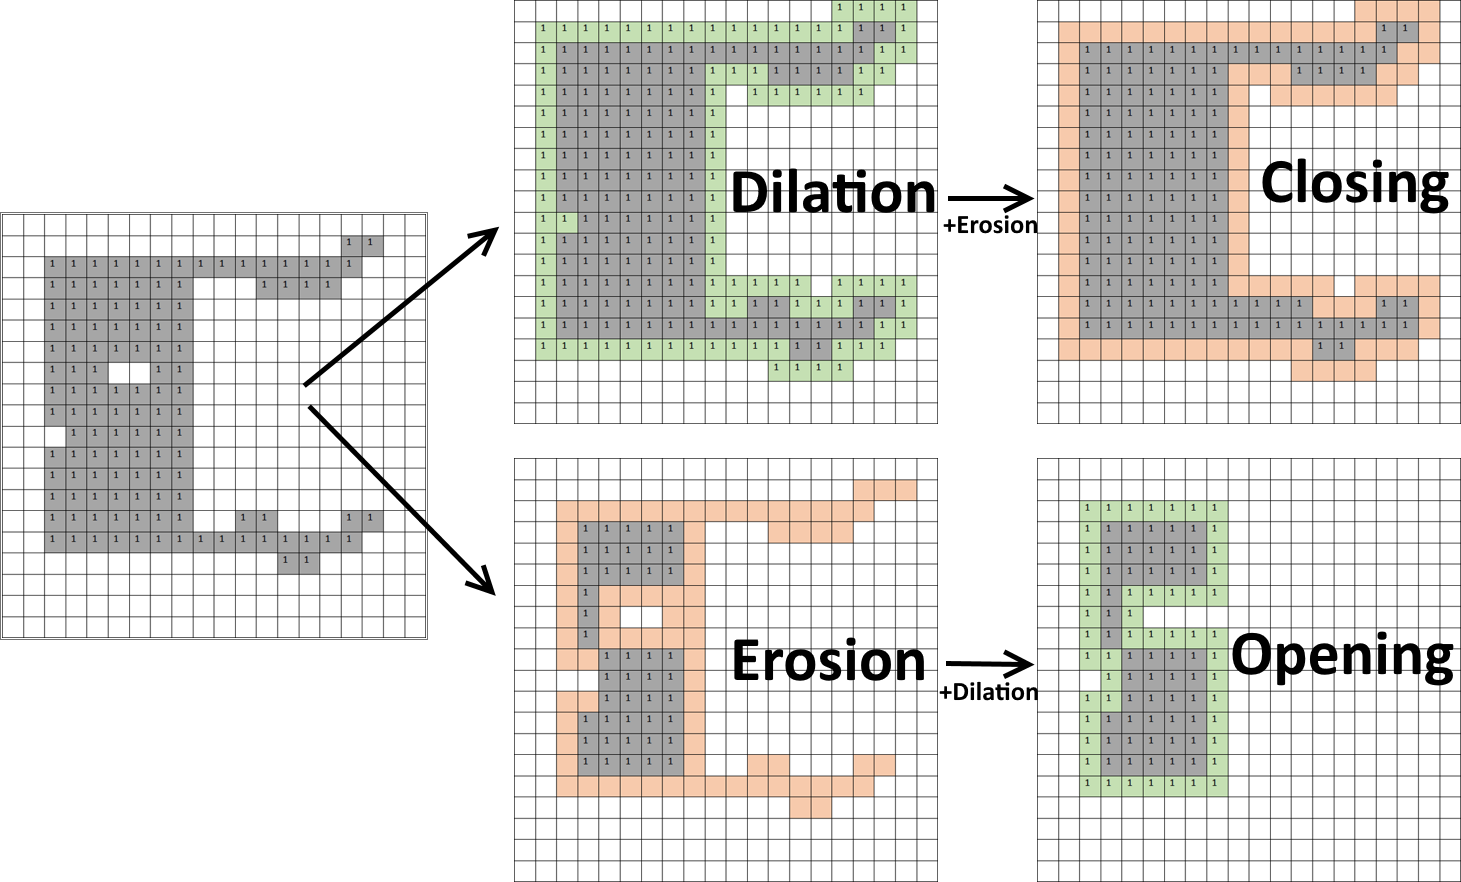
\includegraphics[width=1\textwidth]{media/morph/morph_all_text.png}
 \caption{Morphologische Operationen - Dilation, Erosion, Opening und Closing}
 \label{fig:boxfilter}
\end{figure}

    \chapter{Kalibrierung}
\section{Single-Kamera-Kalibrierung}
\section{Stereokalibrierung}
\section{Rektifizierung}

    \chapter{Background Subtraction}
Definition bzw. Problemstellung \\
Zwei Verfahren mit Framedifference und Tiefpassfiltern -> Problematik Rauschen

    \chapter{Stereoberechnung}
\section{Globale Verfahren}
\section{Lokale Verfahren}
\section{Kombinierte Verfahren}

    \chapter{Segmentierung}

Bei der sogenannten Segmentierung oder auch Clustering geht es darum, aus einer Folge von einzelnen Punkten ein oder mehrere Cluster zu erstellen. Die Entstehung eines solchen Clusters richtet sich dabei nach der Dichte der vorliegenden Punktwolke: Im Bereichen in denen nur wenige Punkte nahe beieinander liegen liegt Rauschen vor und diese Punkte geh\"oren keinem Cluster an. Liegt in einem Bereich jedoch ein hoher Anteil der Gesampunktzahl so sollen diese Punkte als Cluster zusammengefasst werden.

\section{Region Growing Algorithmus}

Der Region-Growing-Algorithmus startet in einem vorgegebenen Gitter an einem vorgegebenen Saatpunkt und arbeitet sich iterativ \"uber das gesamte Bild.

\begin{algorithm}[H]
 \KwData{Binary Image I, Seedpoint p}
 \KwResult{Segmented Image S}
 Queue Q(p) \;
 Label l = 1 \;
 \While{ Q not empty}{
    c = Q.pop() \;
    N = findAllUnvisitedNeighbors(I, S, c) \;
    \eIf{n not empty} {
        MarkPointsAsLabeled(S, l, N) \;
        Q.push(N) \;
    }{
        l++
    }
 }
 \caption{Pseudocode Region-Growing-Algorithmus}
\end{algorithm}


\section{DBScan Algorithmus}

\begin{algorithm}[H]
 \KwData{Point List PL, eps, minPts}
 \KwResult{Segmented Point List S}
 Label l = 1\;
 \ForEach{p in PL} {
    \If{p is labeled}{continue\;}
    N = findAllNeighbors(PL, eps, p) \;
    \If{size(N)<minPts}{label p as noise\; continue\;}
    L++\;
    label p as L \;
    \ForEach{n in N} {
        MarkPointsAsLabeled(S, l, N)\;
        M = findAllNeighbors(PL, eps, n)\;
        \If{size(M)>minPts}{N.push(M)\;}
    }
 }
 \caption{Pseudocode DBSCan-Algorithmus}
\end{algorithm}

\section{Kombinierte Segmentierung}

\begin{algorithm}{H}
 \KwData{Binary Image I, Seedpoint p}
 \KwResult{Segmented Point List S}
 I1 = Downsample(I) \;
 S1 = Segment(I1, p) \;
 S1 = Upsample(S1) \;
 A = ExtractAndJoinAreas(S1) \;
 \ForEach{a in A}{
    pt = ExtractPoints(I, a) \;
    Sk = Segment(pt, eps, minPts) \;
 }
 \caption{Pseudocode Kombinierte Segmentierung}
\end{algorithm}

    \chapter{Klassifikation}

Die Klassifikation besch\"aftigt sich mit der Einordnung von Objekten zu bestimmten Klassen. Die Objekte werden dabei durch einen sogenannten Merkmalsvektor \( x \in \mathbb{R}^n \) beschrieben, welcher definierte Eigenschaften des Objekts enth\"alt. Die benutzten Merkmale k\"onnen je nach Anwendungsfall unterschiedlich ausfallen. Im Bereich der Klassifikation von Verkehrsteilnehmern bieten sich geometrische Eigenschaften wie Ausma\ss{}e des Objekts, Umfang, Volumen oder Dichte an. Die zuzuordnende Klasse oder auch Label genannt ist im Allgemeinen eine ganze Zahl \(y \in \mathbb{Z} \). Der Klassifikator \(f\) l\"asst sich somit beschreiben als:

\begin{equation*}
 f: x \in \mathbb{R}^n \mapsto y \in \mathbb{Z}
\end{equation*}

Er ordnet den Merkmalen eines Objekts eine Klasse zu. Die Form des Klassifikators kann dabei variieren und h\"angt vom Anwendungsfall ab.
F\"ur gew\"ohnlich muss ein Klassifikator trainiert werden. Unter dem Begriff Training versteht man in diesem Zusammenhang den Vorgang, die w\"ahlbaren Parameter der Klassifikationsfunktion so einzustellen, dass er auf einen bestimmten Trainingsdatensatz \( (x_i | y_i)_{i=1..n} \) m\"oglichst gute Daten liefert. Das Training kann als Optimierungsproblem dargestellt werden:
\begin{equation*}
 \min_{\alpha} \sum_{i=1}^n \omega ( f_{\alpha}(x_i), y_i)
\end{equation*}
Die Funktion \( \omega : \mathbb{Z}^2 \mapsto \mathbb{R} \) ist eine Fehlerfunktion welche testet, ob die zu testende Klasse mit der vom Klassifikator ausgewerteten Klasse \"ubereinstimmt:
\begin{equation*}
 \omega (y_1, y_2) = 
 \begin{cases}
  0 & y_1=y_2 \\
  d(y_1, y_2) & y_1 \neq y_2, d>0
 \end{cases}
\end{equation*}

Durch Minimierung der Summe der Fehler kann so eine bestm\"ogliche Approximation an die Trainingsdaten gefunden werden. Im Folgenden werden einige Klassifikatoinsverfahren vorgestellt.

\section{K-Nearest-Neighbor Klassifikation}
Der Nearest-Neighbor-Klassifikator arbeitet ohne einen Optimiegunssprozess direkt auf den Trainingsdaten \( (x_i | y_i)_{i=1..m} \in \mathbb{R}^n \times \mathbb{Z} \). Ein Objekt mit Merkmalen \(b \in \mathbb{R}^n\) wird derjenigen Klasse zugeordnet, zu der der Abstand \(d=\|b-x_i\| \) am geringsten ist:
\begin{equation*}
 f(b)= y_k, k=\underset{{k \in \{1..m\}}}{arg\,min} (||b-x_k||)
\end{equation*}

Die Norm \(\| \cdot \| \) ist hierbei beliebig, h\"aufig wird jedoch die euklidische Norm \(\| \cdot \|_2 \) verwendet.

In Abbildung \ref{fig:classification_knn} ist ein Beispiel f\"ur eine solche Klassifikation zu sehen. Auf der linken Seite wird ein einfacher Nearest-Neighbor-Klassifikator angewendet. Auf der rechten Seite ist jedoch sichtbar, dass das Rauschen in den Daten zu einer Fehlklassifikation f\"uhren w\"urde. Aus diesem Grund wurde der Klassifikator erweitert zum K-Nearest-Neighbor-Klassifikator. Dieser bezieht nicht nur das Trainingsdatum mit dem geringsten Abstand ein, sondern sucht die \(k\) n\"achsten Nachbarn. Das Ergebnis der Klassifikation ist dann diejenige Klasse, welche am h\"aufigsten in dieser Ergebnismenge vorkommt. In der Grafik ist der KNN-Klassifikator f\"ur den fall \(k=3\) dargestellt.

Der KNN-Klassifikator finden h\"aufig zu Testzwecken Anwendung, da er einfach zu implementieren ist und stabile Resultate liefert. Da er kein Training ben\"otigt ist jedoch der Aufwand zur Evaluation hoch und der Algorithmus ist damit nicht sehr effizient. Zu produktiven Zwecken in Echtzeitsystemen wird er daher nur selten verwendet.

\begin{figure}
 \centering
 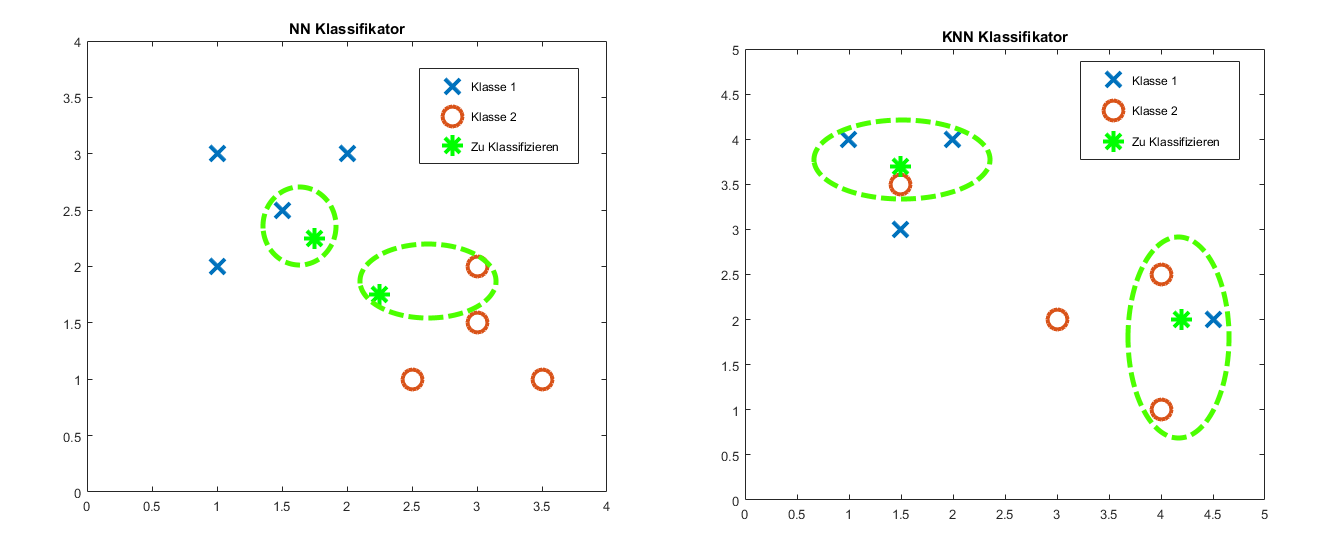
\includegraphics[width=1\textwidth]{media/classification/knn_example.png}
 \caption{Klassifikation - Beispiel f\"ur NN- und KNN-Klassifikator}
 \label{fig:classification_knn}
\end{figure}

\section{Neuronales Netz}
K\"unstliche neuronale Netze sind Modelle, welche biologischen neuronalen Netzen nachempfunden sind. Sie setzen sich aus einer Vielzahl von Neuronen zusammen, welche untereinander verbunden sind und sich gegenseitig beeinflussen bzw. anregen k\"onnen. Ein k\"unstliches neuronales Netz besteht aus einer Eingabeschicht, einem oder mehreren Zwischenschichten und einer Ausgabeschicht. Ein Modell eines solchen Netzes mit einer Zwischenschicht ist in Abbildung \ref{fig:classification_neuralnetwork} zu sehen. Die Eingabeschicht akzeptiert hierbei \(m=4\) Daten als Eingabe, die Zwischenschicht besteht aus \(5\) k\"unstlichen Neuronen und die Ausgabeschicht  liefert ein Ergebnis aus \(n=3\) Ausgabedaten.

\begin{figure}
\centering
\def\layersep{3cm}
\begin{tikzpicture}[shorten >=1pt,->,draw=black!50, node distance=\layersep]
    \tikzstyle{every pin edge}=[<-,shorten <=1pt]
    \tikzstyle{neuron}=[circle,fill=black!25,minimum size=17pt,inner sep=0pt]
    \tikzstyle{input neuron}=[neuron, fill=green!50];
    \tikzstyle{output neuron}=[neuron, fill=red!50];
    \tikzstyle{hidden neuron}=[neuron, fill=blue!50];
    \tikzstyle{annot} = [text width=4em, text centered]

    % Draw the input layer nodes
    \foreach \name / \y in {1,...,4}
    % This is the same as writing \foreach \name / \y in {1/1,2/2,3/3,4/4}
        \node[input neuron, pin=left:\(x_\y\)] (I-\name) at (0,-\y) {};

    % Draw the hidden layer nodes
    \foreach \name / \y in {1,...,5}
        \path[yshift=0.5cm]
            node[hidden neuron] (H-\name) at (\layersep,-\y cm) {};
            
    % Draw the output layer node
    %\node[output neuron,pin={[pin edge={->}]right:y1}, right of=H-3] (O) {};
    \foreach \name / \y in {1,...,3}
        \node[output neuron, pin={[pin edge={->}]right:\(y_\y \)}] (O-\name) at (2*\layersep,-\y-0.5) {};

    % Connect every node in the input layer with every node in the
    % hidden layer.
    \foreach \source in {1,...,4}
        \foreach \dest in {1,...,5}
            \path (I-\source) edge (H-\dest);

    % Connect every node in the hidden layer with the output layer
    \foreach \source in {1,...,5}
        \foreach \dest in {1,...,3}
            \path (H-\source) edge (O-\dest);

    % Annotate the layers
    \node[annot,above of=H-1, node distance=1cm] (hl) {Zwischenschicht};
    \node[annot,left of=hl] {Eingabeschicht};
    \node[annot,right of=hl] {Ausgabeschicht};
\end{tikzpicture}
\caption{Modell eines k\"unstlichen neuronalen Netzes mit einer Zwischenschicht}
\label{fig:classification_neuralnetwork}
\end{figure}

Das Single-Layer-Perzeptron ist das primitivste Netz, welches gebildet werden kann. Es besteht lediglich aus einer Eingabe- und einer Ausgabeschicht. Die Funktion l\"asst sich also wie folgt formulieren:

\begin{equation}
 f_W(x)=\varphi(W \cdot x)
\end{equation}
Der Vektor \(x \in \mathbb{R}^m \) beschreibt die Eingabedaten, die Matrix \(W \in \mathbb{R}^{n \times m} \) enth\"alt die Gewichte der Verbindungen zwischen den Neuronen und die Funktion \(\varphi \) ist die sogenannte Aktivierungsfunktion eines Neurons. Die Aktivierungsfunktion eines Neurons entscheidet, ab welchem Wert ein Neuron angeregt ist oder nicht. Hierbei k\"onnen unterschiedliche Funktionen eingesetzt werden: \\
\begin{tabular}{ll}
 S\"attigungsfunktion & \( \varphi(z)=
\begin{cases}
 0 & z \leq -a \\
 \frac{z}{2a} & -a \leq z \leq a, a \in \mathbb{R} \\
 1 & a \leq z
\end{cases}
\) \\
Fermi-Funktion & \( \varphi(z)=\frac{1}{1+e^{\frac{-z}{a}} }, a \in \mathbb{R} \) \\
Heavyside-Funktion & \(\varphi(z)=
\begin{cases}
 0 & z<0 \\
 1 & z\geq 0
\end{cases} \) \\
Lineare Funktion & \( \varphi(z) = a \cdot z \)
\end{tabular}

Im Allgemeinen wird vorausgesetzt, dass alle Neuronen einer Schickt die gleiche Aktivierungsfunktion besitzen.
F\"ur gew\"ohnlich bestehen neuronale Netze aus mehreren Schichten Perzeptronen. Die einzelnen Ergebnisse der Schichten werden nun nacheinander verkn\"upft um so das Ergebnis der Ausgabeschicht zu erhalten:
\begin{equation}
 f_W(x) = \varphi_k(W_k \cdot \varphi_{k-1}(W_{k-1} \cdot \varphi_{k-2}(... \cdot \varphi_1(W_1x)...)))
\end{equation}
Die Matrizen \(W_k\) repr\"asentieren hierbei die Gewichte der Kanten der einzelnen Schichten. Die Gr\"o\ss{}e h\"angt als von der Anzahl der Neuronen in der jeweiligen Schicht ab. Ebenso kann sich die Aktivierungsfunktion \( \varphi_k\) der einzelnen Schichten unterscheiden.

Beim Training eines neuronalen Netzes werden die Gewichte \(W_k\) bestimmt. Hierzu ist wiederum ein Trainingsdatensatz notwendig: 
 \( (x_k | y_k)_{k=1..r} \in \mathbb{R}^m \times \mathbb{R}^n \)
Der eigentliche Trainigsvorgang soll die Gewichte so bestimmen, dass der quadratische Fehler der Klassifikation minimiert wird:
\begin{equation}
 \underset{W}{min} \sum_{k=1}^r \sum_{j=1}^n (f_W(x_j^k)-y_j^k)^2
\end{equation}
Hierbei handelt es sich um ein unrestringiertes Optimierungsproblem, da an die zu optimierende Variable \(W\) keine Nebenbedingungen gekn\"upft sind. Zum L\"osen des Optimierungsproblems existieren diverse Verfahren. Welches Verfahren eingesetzt wird h\"angt von der Zusammensetzung des Netzes und der Wahl der Aktivierungsfunktion zusammen. Ist die resultierende Funktion linear k\"onnen schnellere Verfahren wie die QR-Zerlegung oder das CG-Verfahren eingesetzt werden. Im nichtlinearen Fall sind m\"ogliche Verfahren das Gradientenverfahren, das Newtonverfahren oder auch das Levenberg-Marquardt-Verfahren.

\section{Support Vector Machine}
Die Klassifikation durch die sogenannte Support Vector Machine wird vorallem f\"ur bin\"are Klassifikationsprobleme verwendet. Ziel der Methode ist es, eine Hyperebene zu finden, welche zwei linear trennbare Mengen voneinander trennt. Der Klassifikator hat die Form
\begin{equation*}
 f_{w, b}(x) = 
 \begin{cases}
  1 & w^\intercal x+b>0 \\
  0 & sonst
 \end{cases}
\end{equation*}
 Der Vektor \(w \in \mathbb{R}^n \) ist die Normale der Ebene, das Skalar \(b \in \mathbb{R}\) ist der sogenannte Bias, also die Verschiebung. Diese beiden Parameter m\"ussen durch das Training des Klassifikators berechnet werden. Hierzu wird das Optimierungsproblem anhand der Trainingsdaten \( (x_i | y_i)_{i=1..m} \in \mathbb{R}^n \times \mathbb{Z} \) formuliert:
\begin{eqnarray*}
 & \min \frac{1}{2}||w||_2^2 \\
 & y_i(w^\intercal x_i+b) \geq 1, \forall (x_i | y_i)
\end{eqnarray*}
Die Nebenbedingung fordert hierbei, dass beide Klassen tats\"achlich linear trennbar sind. Da dies im Allgemeinen nicht der Fall ist wird eine sogenannte Schlupfvariable eingef\"ugt, welche die Verletzung der Nebenbedingung erlaubt:
\begin{eqnarray*}
 &\min \frac{1}{2}||w||_2^2+C \sum_{i=1}^m \xi_i \\
 &y_i(w^\intercal x_i+b) \geq 1-\xi_i, \forall (x_i | y_i)
\end{eqnarray*}

In Abbildung \ref{fig:classification_svmlinear} ist eine lineare Trennebene zu sehen. Die Methode der Support Vector Machine erm\"oglicht neben einer linearen auch eine nichtlineare Trennebene, was in Abbildung \ref{fig:classification_svmnonlinear} zu sehen ist. Das Optimierungsproblem gestaltet sich dabei deutlich komplexer, weshalb in dieser Arbeit auf die lineare Variante zur\"uckgegriffen wird.

\begin{figure}
\centering
\begin{minipage}{.5\textwidth}
  \centering
  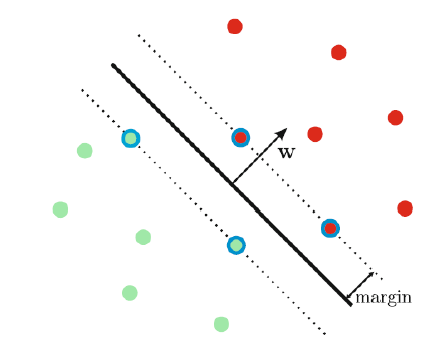
\includegraphics[width=1\textwidth]{media/classification/svm_linear.png}
  \captionof{figure}{SVM linear}
  \label{fig:classification_svmlinear}
\end{minipage}%
\begin{minipage}{.5\textwidth}
  \centering
  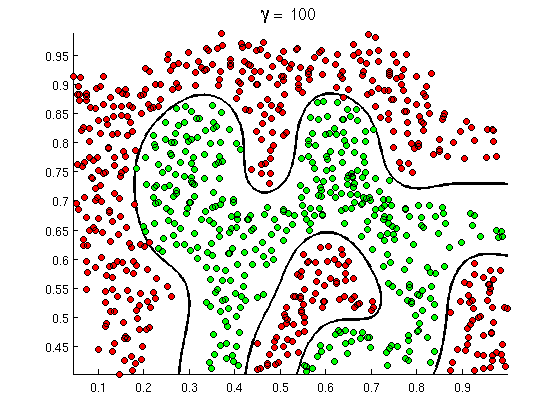
\includegraphics[width=1\textwidth]{media/classification/svm_nonlinear.png}
  \captionof{figure}{SVM nichtlinear}
  \label{fig:classification_svmnonlinear}
\end{minipage}
\end{figure}

    \chapter{Tools und Datensatze}

\section{Background Subtraction Datasets}
\subsection*{ChangeDetection.NET}
Der changedetection Datensatz ist eine im Jahr 2012 Ö entstandene Sammlung von Videos, welche unterschiedliche Szenarien und Kameraeigenschaften darstellen. Die Motivation der Urheber ist, dass kein universeller Algorithmus existiert, welcher alle Szenarien angemessen gut auswerten kann. Im Datensatz vorhandene Szenarien sind:
\begin{multicols}{2}
Datensatz 2012:
\begin{itemize}
 \item Dynamischer Hintergrund
 \item Wackelnde Kamera
 \item Unregelm\"aßge Objektbewegungen
 \item Schatten
 \item W\"armebildkameras
\end{itemize}

\columnbreak

Datensatz 2014:
\begin{itemize}
 \item Wettereinfluss
 \item Niedrige Bildrate
 \item Nachtaufnahmen
 \item \"Uberwachungskameras
 \item Luftturbulenzen durch thermische St\"orungen
\end{itemize}
\end{multicols}

Ebenso mitgeliefert werden zu den Videos geh\"orige Ground-Truth-Daten, welche die tats\"achliche Bewegung in den einzelnen Bildern beschreiben. Diese Daten wurden mitunter manuell erstellt. Als Vordergrund gelten unter anderem Regionen, welche nicht Teil des statischen Hintergrunds sind und bei denen es sich insbesondere um Objekte wie Personen oder Fahrzeuge handelt. Auch Objekte, die eine kurze Standzeit im Bild haben, sollen nicht als Hintergrund klassifiziert werden. Dagegen werden St\"orungen wie Lichtreflexion, Schatten oder Turbulenzen in der Luft nicht als Vordergrnud detektiert. 


\subsection*{Background Model Challenge}

Der Datensatz der Background Model Challenge (BMC) enth\"alt eine Sammlung an Videos, welche ebenfalls zur Evaluation von Background-Detection-Algorithmen benutzt werden k\"onnen. Hierzu ist eine Reihe von unterschiedlichen Videosqeuenzen vorhanden, welche verschiedene Szenen abbilden. Der Unterschied zum oben beschriebenen changedetection-Datensatz ist, dass auch synthetische Videos zur Verf\"ugung stehen. Dies sind Videos, welche durch das Rendern einer aufgebauten 3D-Szene am Computer erstellt wurden. Der Vorteil dieses Vorgehens ist, dass die zugeh\"origen Ground-Truth-Daten direkt mit erzeugt werden k\"onnen und keine aufw\"andige Nachbearbeitung n\"otig ist. Daf\"ur werden jedoch in der Praxis auftretende Effekte vernachl\"assigt, wie beispielsweise eine sich bewegende Kamera oder Turbulenzen. Die synthetischen Videos sind daher nur bedingt nutzbar.

\section{Stereo Datens\"atze}
\subsection*{Kitti Datensatz}


Der Kitti Datensatz ist eine mfangreiche Sammlung von Dates\"atzen, welche im Zusammenhang mit autonomem Fahren verwendet werden. So sind unter anderem Datens\"atze vorhanden f\"ur Stereovision, Szenenfluss oder Objekt-Tracking vorhanden. Die Videodaten sowie zugeh\"orige Ground-Truth-Daten wurden mit Hilfe eines Sensorfahrzeugs erzeugt, welches mit Lidar und GPS ausger\"ustet ist. Die Sequenzen wurden sowohl innerhalb wie au\ss{}erhalb von St\"adten aufgenommen und enthalten eine ausreichende Anzahl an Fahrzeugen und Fu\ss{}g\"angern. Zus\"atzlich zu den Ground-Truth-Daten sind auch Benchmarks und Evaluationsalgorithmen vorhanden um angewendete Algorithmen vergleichbar zu machen. Die Seite bietet auch die M\"oglichkeit der Einreichung von Algorithmen und listet diese geordnet nach ihrer Effektivit\"at auf.

Der Kitti Datensatz hat besondere Relevanz f\"ur diese Arbeit, da sich die Szenerie ausschlie\ss{}lich auf den Stra\ss{}enverkehr konzentriert. Nachteilig ist, dass pro Szene nur zwei Bilder vorhanden sind und somit keine kontinuierliche Verkehrsszene abgebildet wird. 
\subsection*{Stereo Ego-Motion Dataset}

Der Stereo Ego-Motion Datensatz enth\"alt 494 hochaufl\"osende Videos von vier Objekten: Eine Auto, eine Katze, ein Stuhl und ein Hund. Im Video werden diese Objekte  mit der Kamera umkreist um ein Rundumbild zu erzeugen. Dazu sind ebenfalls Ground-Truth-Daten vorhanden. Mit diesem Vorgehen k\"onnen komplette 3D-Meshes anhand der Stereodaten erzeugt werden. F\"ur das einfache Benchmarking von Stereodaten ist der Datensatz auch zu verwenden, wobei die Eigenkamerabewegung nur bedingt zum Thema der Arbeit passt. 

\subsection*{Middlebury Stereo Dataset}

Der Middlebury Datensatz enth\"alt f\"und verschiedene Datens\"atze mit insgesamt 71 unterschiedlichem Motiven. Enthalten sind Ground-Truth-Daten sowie ein Softwaretool zur Evaluation. Auch das Einreichen erzielter Ergebnisse ist m\"oglich. Besonders interessant an diesem Datensatz ist, dass die Objekte unter variablen Lichtverh\"altnissen aufgenommen wurden. So stehen zu jedem Objekt Bilder mit vier unterschiedlichen Beleuchtungen. Dies stellt den Stereoalgorithmus zus\"atzlich vor Herausforderungen, da auch in der Realit\"at und vorallem im Stra\ss{}enverkehr Licht eine bedeutende Rolle spielt.


\newpage
\section{Tools}
\subsection*{OpenCV}
OpenCV ist eine offene Softwarebibliothek f\"ur die Sprache C++, die auf den Bereich der maschinellen Bildverarbeitung spezialisiert ist. In OpenCV sind mehr als 2500 Algorithmen vorhanden. Am Projekt beteiligen sich laut eigenen Angaben mehr als 47000 Entwickler und die gesch\"atze Downloadzahl liegt bei ca. 14 Millionen \cite{opencv}. Einen \"Uberblick \"uber die Kernfunktionalit\"at der Bibliothek gibt folgende Liste \cite{opencv_nvidia, opencv_wikipedia}:

\begin{itemize}
 \item Bild- und Videoverarbeitung und Darstellung
 \item Objekterkennung und Extraktion von Objektmerkmalen
 \item Kamerakalibrierung und Stereovision
 \item Maschinelles Lernen und Clusteringverfahren
 \item Eigenbewegungssch\"atzung
 \item Gesichts- und Gestenerkennung
\end{itemize}
 OpenCV ist sehr effizient und wird produktiv in der Industrie eingesetzt. So setzen sowohl offene Softwareprojekte oder Startups auf OpenCV, aber auch gr\"o\ss{}ere Firmen wie Google, Microsoft oder Yahoo sind vertreten. Die Einsatzgebiete reichen dabei von der Verkehrs\"uberwachung \"uber Roboternavigation bis hin zur Gesichtserkennung in Japan. 
 
 OpenCV kann dabei nicht nur in C++ zum Einsatz kommen: Es sind auch Schnittstellen zu Python, Java und Matlab verf\"ugbar, wobei alle g\"angigen Betriebssysteme unterst\"utzt werden.
\subsection*{CUDA}

\subsection*{Point Cloud Library}
\subsection*{Javascript Object Notation}

    \chapter{Evaluation Background Subtraction}

    \chapter{Evaluation Stereoberechnung}

    \chapter{Fahrzeugdetektion}



\section{Programmablauf}

\begin{figure}
 \centering
 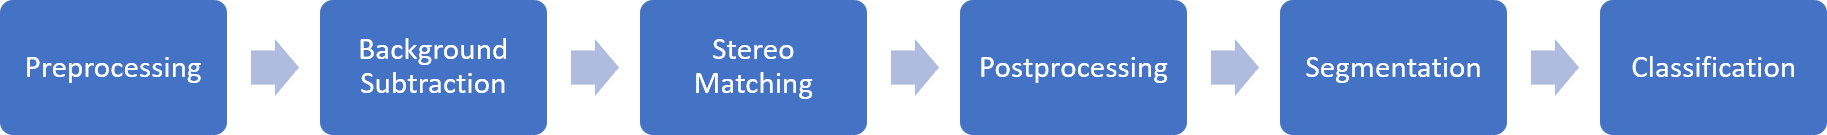
\includegraphics[width=1.1\textwidth]{media/pipeline.png}
 \caption{Pipeline zur Detektion}
 \label{fig:detection_programpipeline}
\end{figure}

\begin{figure}
 \centering
 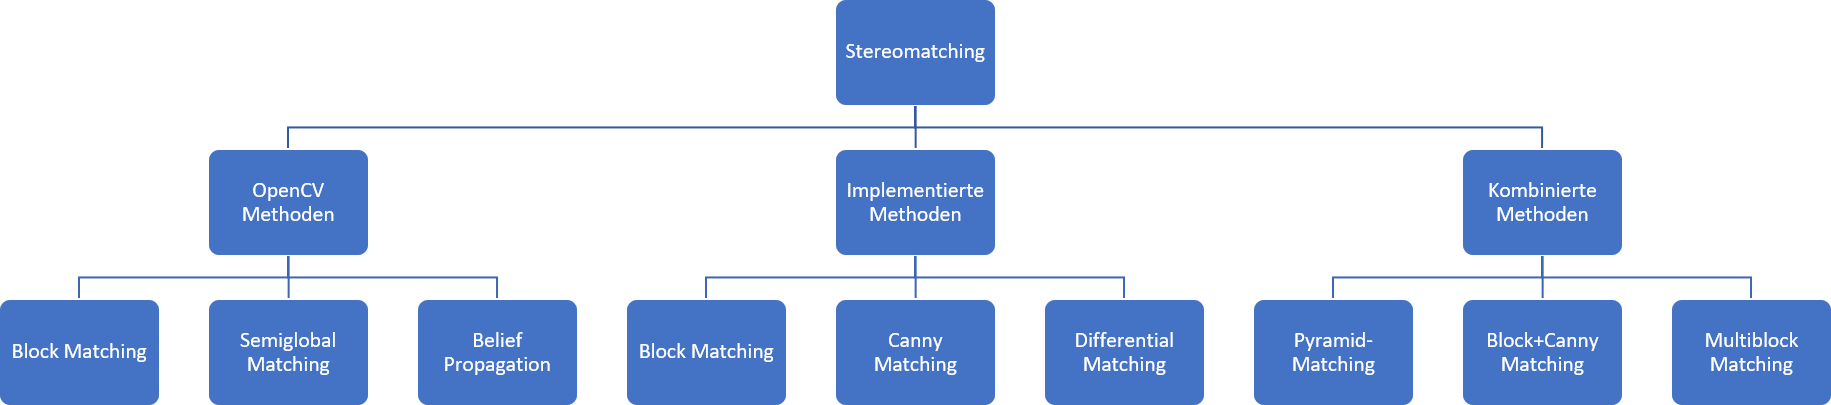
\includegraphics[width=1.1\textwidth]{media/detection/stereomatcher.png}
 \caption{Pipeline zur Detektion}
 \label{fig:detection_stereomatcher}
\end{figure}

\section{3D-Grafik}
\begin{figure}
 \centering
 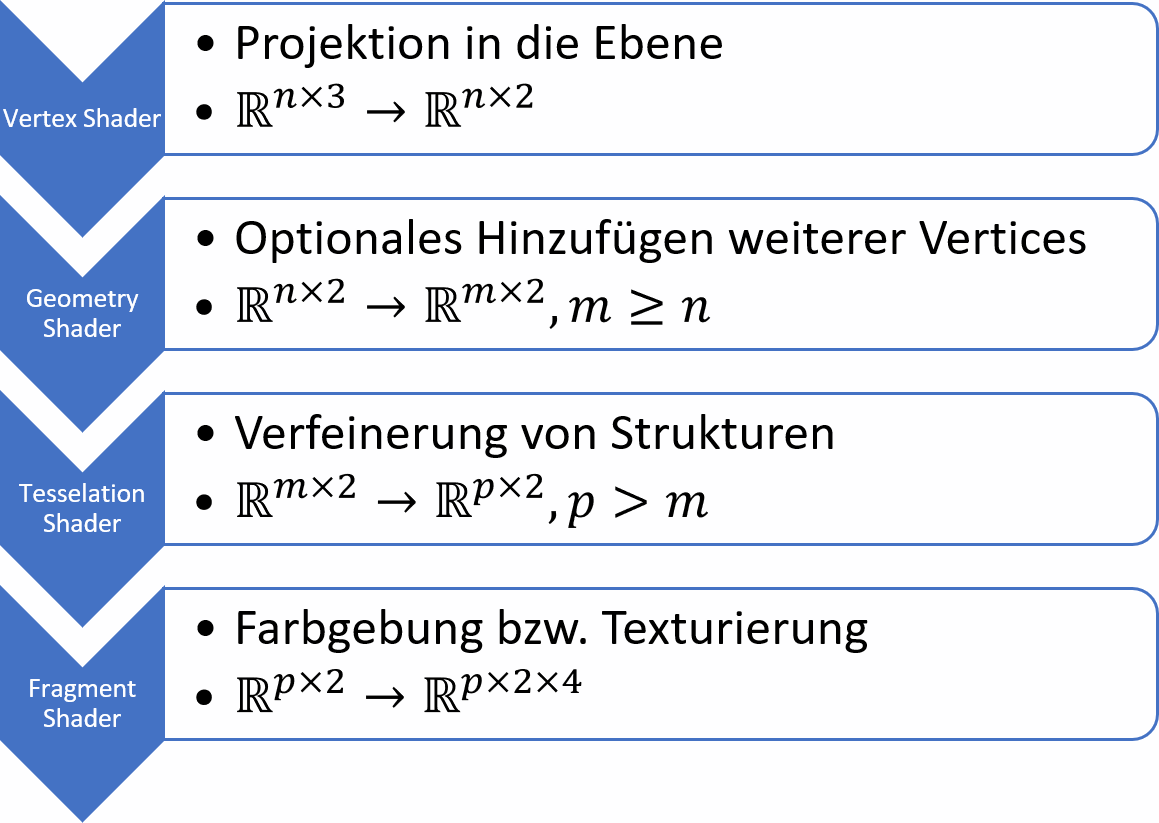
\includegraphics[width=1.1\textwidth]{media/detection/graphics_pipeline.png}
 \caption{Pipeline zur Detektion}
 \label{fig:detection_graphicspipeline}
\end{figure}

\section{Evaluation}

\subsection{Fehlernormen}

\(d_C(x, y) \) berechnete Disparity Map
\(d_T(x, y) \) Ground Truth Map

Bad Pixel Percentage

\begin{equation}
 P = \frac{1}{N} \sum_{(x, y)}(|d_C(x, y)-d_T(x, y)|>\delta_d)
\end{equation}

\(\delta_d \) Fehlertoleranz

Root Mean Squared Error
\begin{equation}
 E = \bigg( \frac{1}{N}\sum_{(x, y)}|d_C(x, y)-d_T(x, y)|^2 \bigg)^{\frac{1}{2}}
\end{equation}

   
   %\input{doc/}
   %\input{doc/}
% - - - - - - - - - - - - - - -
  \appendix                        %import all your appendix stuff here
   %\input{doc/}
   %\input{doc/}
% - - - - - - - - - - - - - - -
  \backmatter
%  \nocite{*} %add all items of bib file to bibliography. Replace "*" by a list of specific
%             % bibentry keys to select only some, or comment this line
%             %normally, all bib entries should be cited in the text
   \printbibliography[heading=bibintoc]
% - - - - - - - - - - - - - - -
\end{document}                      %yeah, you're done
